	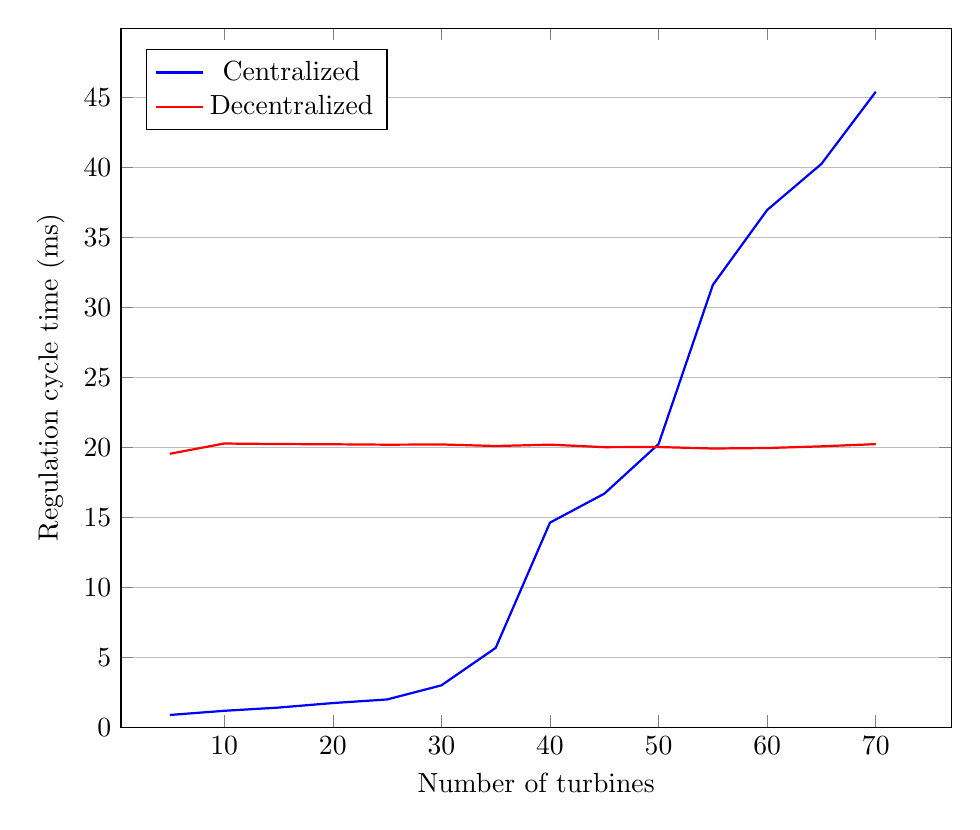
\begin{tikzpicture}
	
	\begin{axis}[%
	width=\resultsPlotWidthScale\textwidth,
	xmin=0.5,
%	xmax=20.5,
	xlabel=Number of turbines,
	ylabel=Regulation cycle time (ms),
%	xtick={1, 2, 3, 4, 5, 6, 7, 8, 9, 10, 11, 12, 13, 14, 15, 16, 17, 18, 19},
%	xticklabels={ 5, , 15, , 25, , 35, , 45, , 55, , 65, , 75, , 85, , 95},
	ymin=0,
	%	ymax=300,
	ymajorgrids=true,
%	yminorgrids=true,
%	max space between ticks=17.5,
	legend entries={Centralized,Decentralized},
	legend style={
		legend pos= north west,
	}
	]
	
	\addplot[thick, blue] coordinates {
		(5 ,0.871522)
		(10 ,1.168815)
		(15 ,1.398871)
		(20 ,1.722236)
		(25 ,1.978881)
		(30 ,2.985681)
		(35 ,5.662268)
		(40 ,14.607313)
		(45 ,16.673738)
		(50 ,20.220936)
		(55 ,31.587407)
		(60 ,36.93711)
		(65 ,40.231022)
		(70 ,45.380062)
%		(75 ,51.425649)
%		(80 ,58.196177)
%		(85 ,64.70376)
%		(90 ,73.715686)
%		(95 ,82.961949)
	};
	
	\addplot[thick, red] coordinates {
		(5 ,19.526002) 
		(10 ,20.257002)
		(15 ,20.221001)
		(20 ,20.203002)
		(25 ,20.174001)
		(30 ,20.190001)
		(35 ,20.079)
		(40 ,20.176)
		(45 ,19.998)
		(50 ,20.008)
		(55 ,19.902002)
		(60 ,19.937001)
		(65 ,20.056)
		(70 ,20.215)
%		(75 ,19.920001)
%		(80 ,20.129002)
%		(85 ,20.189001)
%		(90 ,20.902001)
%		(95 ,27.909001)
%		(100 ,43.314001)
	};
	\end{axis}
	\end{tikzpicture}